% cos-impl.tex

\documentclass[tikz]{standalone}
\usepackage{amsmath, amsfonts}
\usetikzlibrary{positioning, shapes, decorations.pathreplacing, fit}

\begin{document}
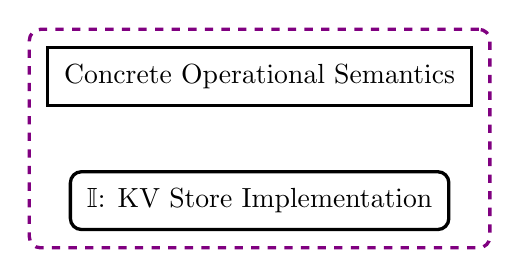
\begin{tikzpicture}[rect/.style = {draw, very thick, rectangle, inner sep = 6pt}, % rectangle
  rrect/.style = {rect, rounded corners}, % rounded rectangle
  refine/.style = {very thick, teal, ->}
]
  \node (impl) [rrect] {$\mathbb{I}$: KV Store Implementation};
  \node (cos) [rect, above = 0.80cm of impl] {Concrete Operational Semantics};
  \node (impl-cos) [draw, violet, inner sep = 6pt, fit = (impl) (cos), very thick, dashed, rectangle, rounded corners] {};
\end{tikzpicture}
\end{document}
